
\documentclass[12pt]{article}
\usepackage[arabic]{babel}
\usepackage[utf8]{inputenc}
\usepackage{amssymb}
\usepackage{geometry}
\usepackage{graphicx}
\usepackage{wrapfig}
\usepackage{amsmath}
\usepackage{lipsum}
\usepackage{caption}
\usepackage{ulem}
\usepackage{xcolor}
\usepackage{polyglossia}
\usepackage{tikz}
\usetikzlibrary{arrows.meta, positioning, shapes}
\setdefaultlanguage{arabic}
\setotherlanguage{english}

% Font and layout settings
\newfontfamily\arabicfont[Script=Arabic,Scale=1.2]{Amiri}
\geometry{top=2cm, bottom=2cm, left=2cm, right=2cm}

% Colors
\definecolor{titleColor}{HTML}{800000} % Maroon for titles
\definecolor{sectionColor}{HTML}{4682B4} % SteelBlue for sections
\definecolor{textHighlight}{HTML}{DAA520} % Goldenrod for highlights
\definecolor{backgroundColor}{HTML}{F0F8FF} % AliceBlue background
\definecolor{emphasisColor}{HTML}{228B22} % ForestGreen for emphasis

% Page styling
\pagecolor{backgroundColor}
\color{black}

\begin{document}

\begin{center}
{\Huge\textbf{\textcolor{titleColor}{السودان  الحرب والسلام الاستقرار والازدهار }}}
    \vspace{0.5cm}
    \textbf{\textcolor{emphasisColor}{بابكر عثمان}} \\
    \vspace{0.2cm}
    \today
\end{center}


\begin{wrapfigure}{r}{0.40\textwidth}
\rotatebox{0}{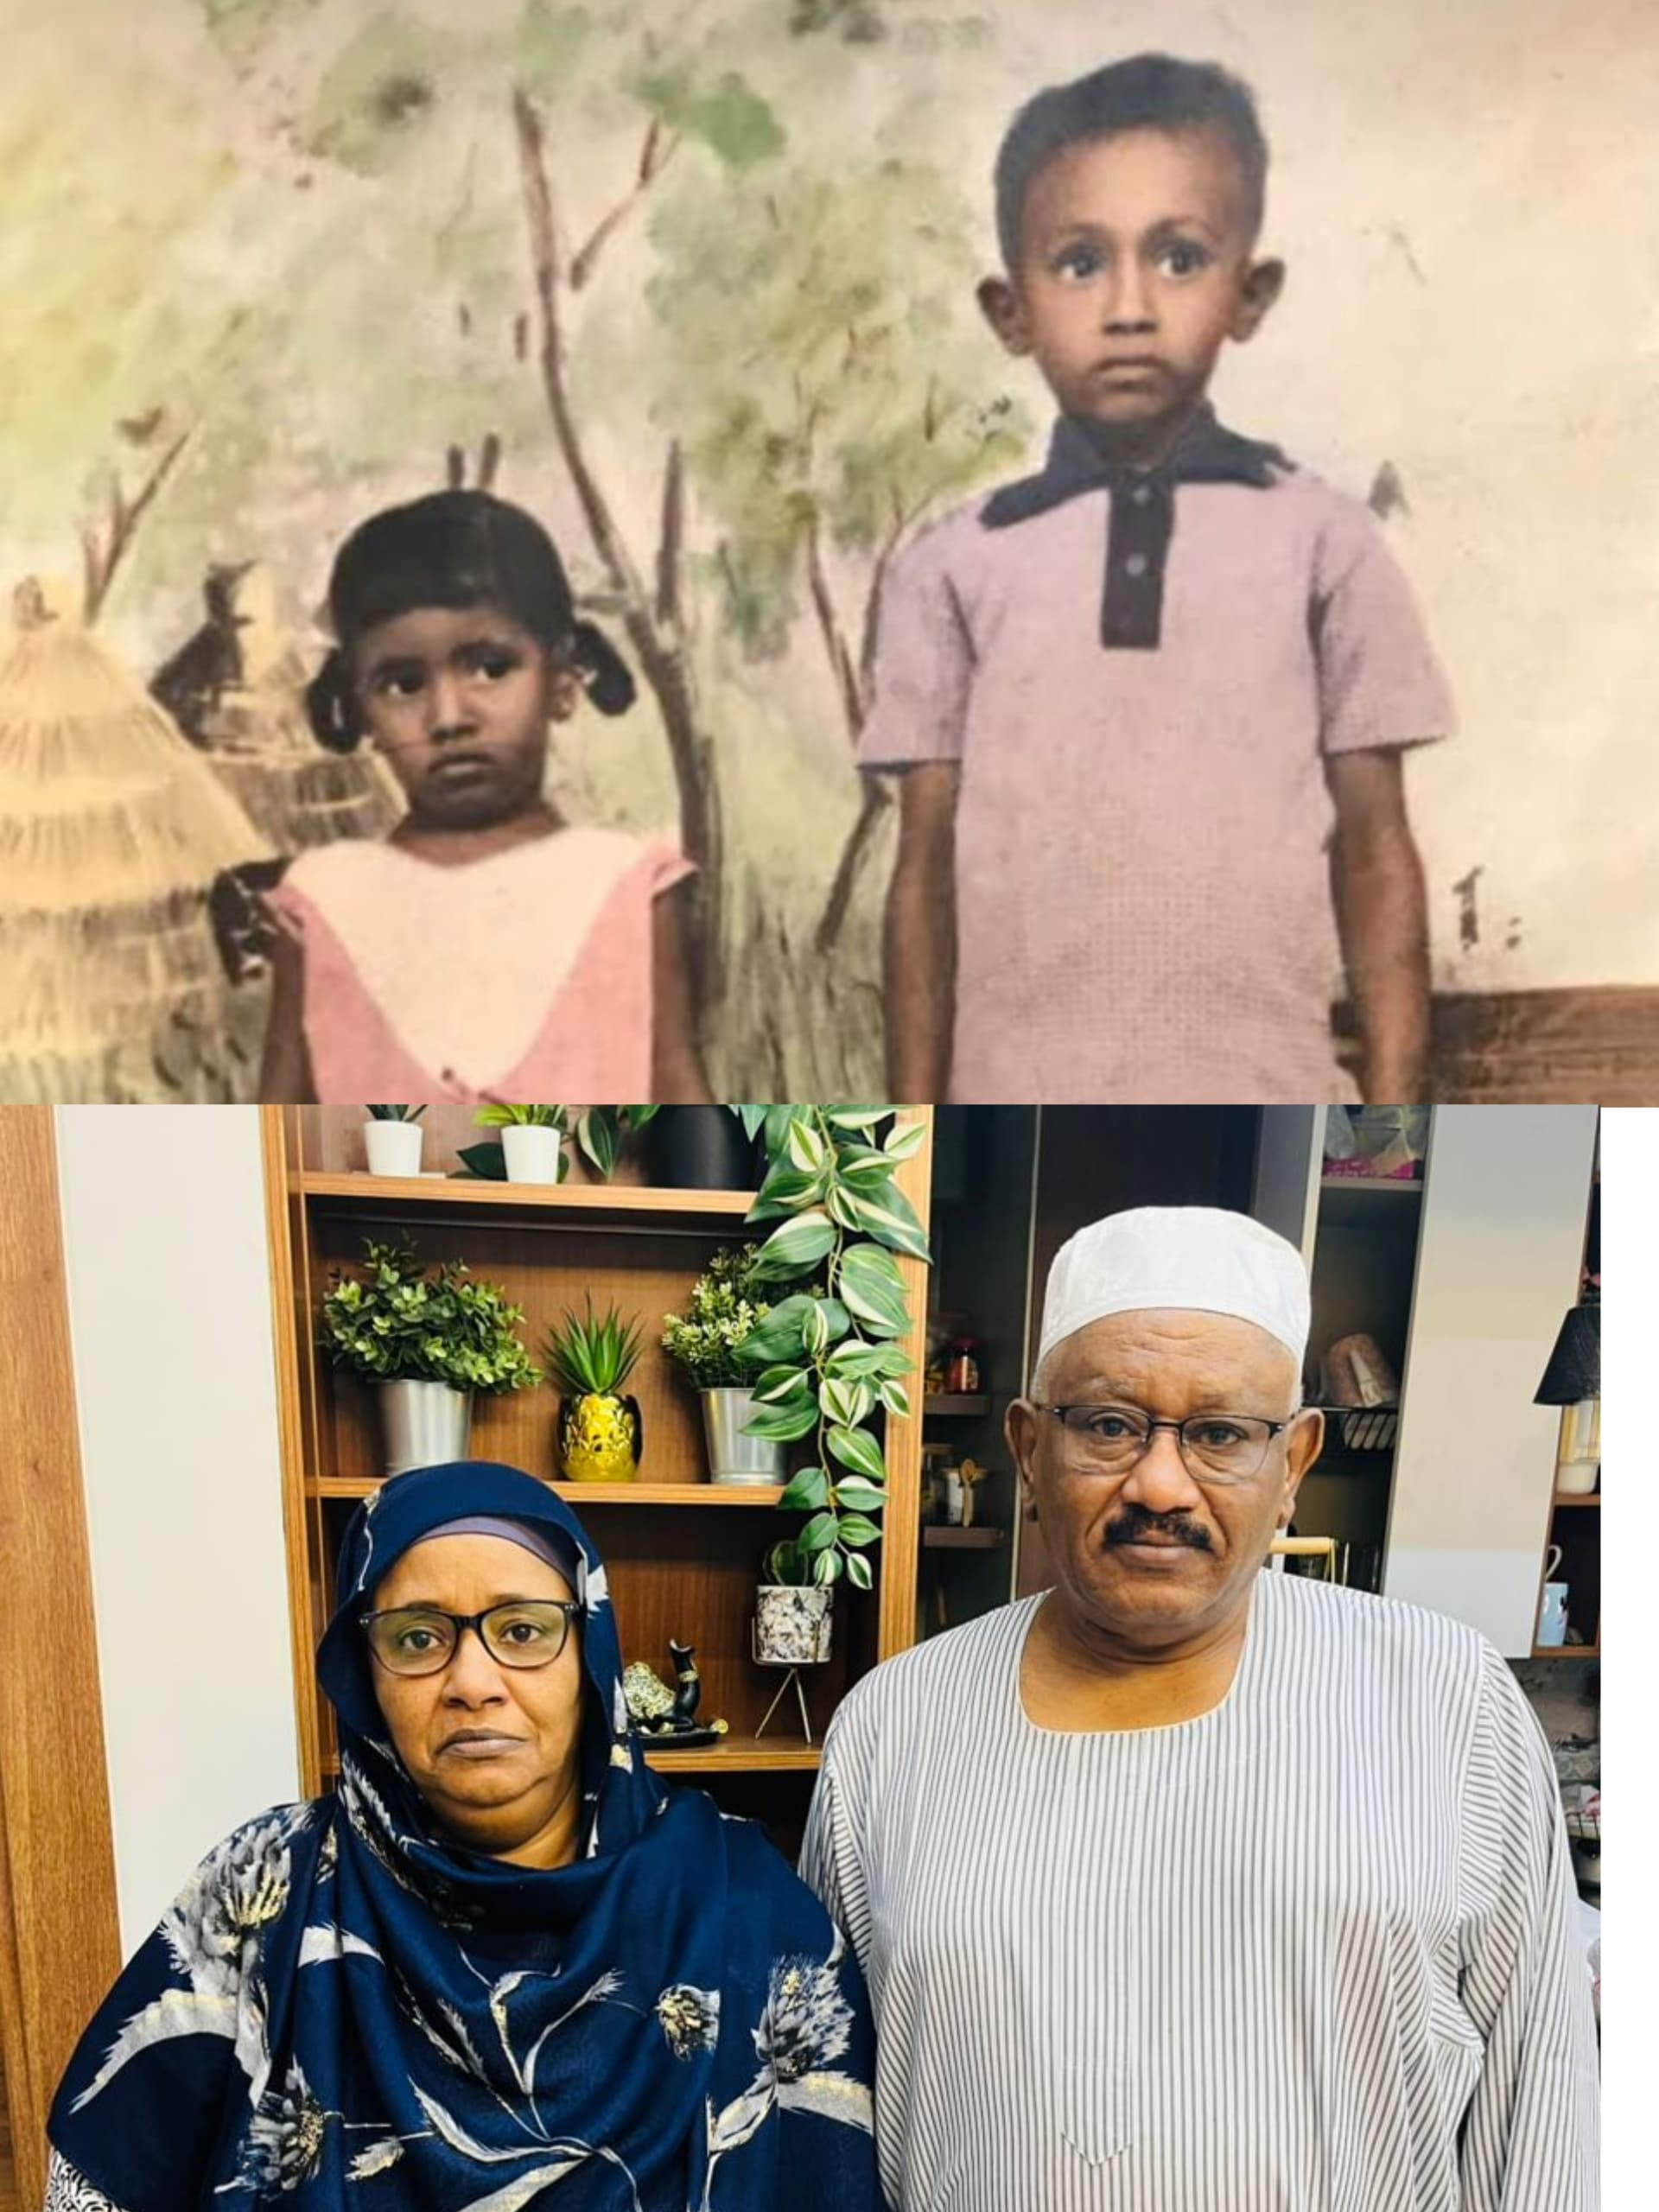
\includegraphics[width=0.4\textwidth]{205.jpg}}

\caption{اطفال الماضى اجداد اليوم  }
\end{wrapfigure}



إلى أختي وأخي، أطفال السبعينات، الآن أجداد \\

يا طفولةَ السبعيناتِ في أمانِ \\
نسجتُم الأملَ في قلبِ الزمانِ \\
لعبتُم على الترابِ بلا قيودٍ \\
وأحلامُكم كانت مثلَ الأماني \\

كانت الأيامُ تحنو بابتسامةٍ \\
وساعاتُ النهارِ طُولُ الأماني \\
لا هاتفَ يُلهي، لا شاشاتِ نورٍ \\
بساطُ الأرضِ عالمكم بأمانِ \\

واليومَ قد كبرتم وزاد النورُ فيكم \\
وأنتمُ الآنَ مصدرُ الألحانِ \\
جدودٌ أنتم، وذِكرى الماضي حُلوةٌ \\
تُحكى للصغارِ بكل امتنانِ \\

يا أختي، يا أخي، يا حكاياتِ الأمسِ \\
حِكمتُكم تنيرُ الدربَ للزمانِ \\
فالزمنُ يمضي، لكنَّ الأرواحَ باقيةٌ \\
تحملُ الحبَّ والوصلَ في المكانِ \\

أنتم تاريخُنا ومجدُنا الأصيلُ \\
تعيشونَ في القلوبِ بكل ألوانِ \\
فاحكوا حكاياكم للصغارِ دوماً \\
علَّهم يروا العظمةَ في الإنسانِ. \\

\end{document}

